% Created by tikzDevice version 0.12 on 2019-03-10 18:28:25
% !TEX encoding = UTF-8 Unicode
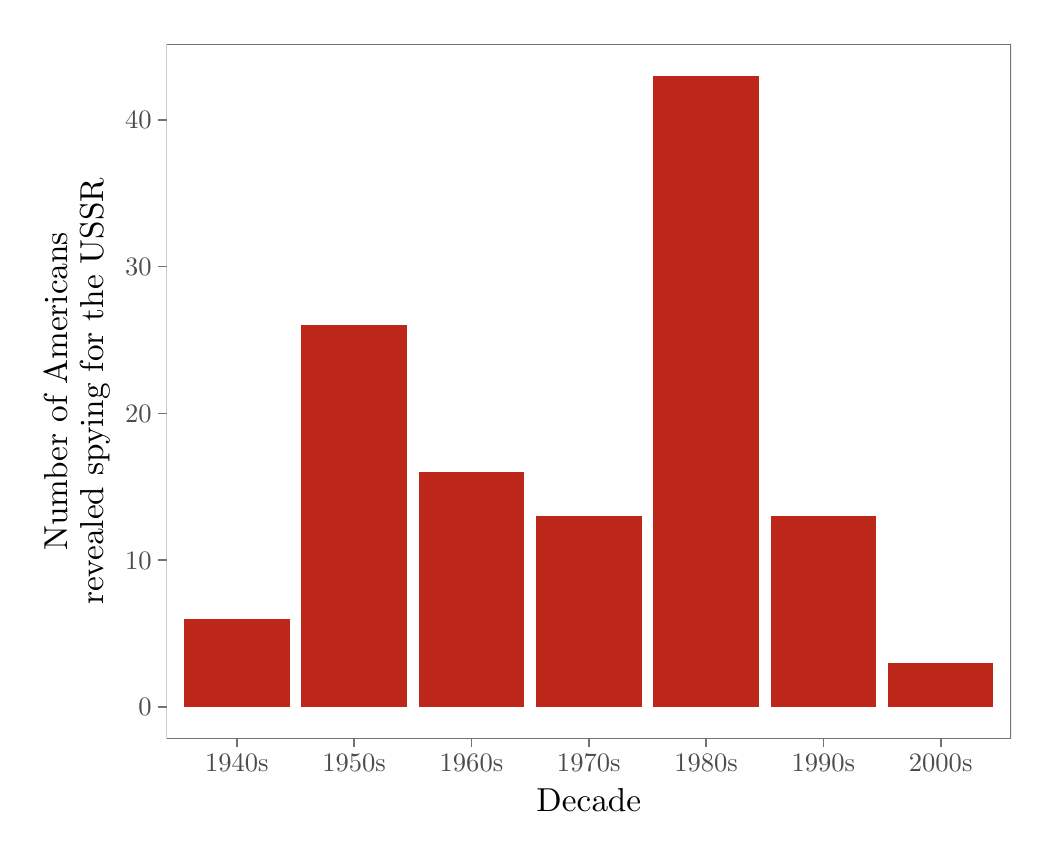
\begin{tikzpicture}[x=1pt,y=1pt]
\definecolor{fillColor}{RGB}{255,255,255}
\path[use as bounding box,fill=fillColor,fill opacity=0.00] (0,0) rectangle (361.35,289.08);
\begin{scope}
\path[clip] (  0.00,  0.00) rectangle (361.35,289.08);
\definecolor{drawColor}{RGB}{255,255,255}
\definecolor{fillColor}{RGB}{255,255,255}

\path[draw=drawColor,line width= 0.6pt,line join=round,line cap=round,fill=fillColor] (  0.00,  0.00) rectangle (361.35,289.08);
\end{scope}
\begin{scope}
\path[clip] ( 50.17, 32.28) rectangle (355.35,283.08);
\definecolor{fillColor}{RGB}{255,255,255}

\path[fill=fillColor] ( 50.17, 32.28) rectangle (355.35,283.08);
\definecolor{fillColor}{RGB}{188,39,26}

\path[fill=fillColor] ( 56.52, 43.68) rectangle ( 94.67, 75.49);

\path[fill=fillColor] ( 98.91, 43.68) rectangle (137.06,181.54);

\path[fill=fillColor] (141.30, 43.68) rectangle (179.45,128.51);

\path[fill=fillColor] (183.68, 43.68) rectangle (221.83,112.61);

\path[fill=fillColor] (226.07, 43.68) rectangle (264.22,271.68);

\path[fill=fillColor] (268.46, 43.68) rectangle (306.61,112.61);

\path[fill=fillColor] (310.84, 43.68) rectangle (348.99, 59.58);
\definecolor{drawColor}{gray}{0.45}

\path[draw=drawColor,line width= 0.6pt,line join=round,line cap=round] ( 50.17, 32.28) rectangle (355.35,283.08);
\end{scope}
\begin{scope}
\path[clip] (  0.00,  0.00) rectangle (361.35,289.08);
\definecolor{drawColor}{gray}{0.30}

\node[text=drawColor,anchor=base east,inner sep=0pt, outer sep=0pt, scale=  0.96] at ( 44.77, 40.37) {0};

\node[text=drawColor,anchor=base east,inner sep=0pt, outer sep=0pt, scale=  0.96] at ( 44.77, 93.39) {10};

\node[text=drawColor,anchor=base east,inner sep=0pt, outer sep=0pt, scale=  0.96] at ( 44.77,146.42) {20};

\node[text=drawColor,anchor=base east,inner sep=0pt, outer sep=0pt, scale=  0.96] at ( 44.77,199.44) {30};

\node[text=drawColor,anchor=base east,inner sep=0pt, outer sep=0pt, scale=  0.96] at ( 44.77,252.47) {40};
\end{scope}
\begin{scope}
\path[clip] (  0.00,  0.00) rectangle (361.35,289.08);
\definecolor{drawColor}{gray}{0.45}

\path[draw=drawColor,line width= 0.6pt,line join=round] ( 47.17, 43.68) --
	( 50.17, 43.68);

\path[draw=drawColor,line width= 0.6pt,line join=round] ( 47.17, 96.70) --
	( 50.17, 96.70);

\path[draw=drawColor,line width= 0.6pt,line join=round] ( 47.17,149.72) --
	( 50.17,149.72);

\path[draw=drawColor,line width= 0.6pt,line join=round] ( 47.17,202.75) --
	( 50.17,202.75);

\path[draw=drawColor,line width= 0.6pt,line join=round] ( 47.17,255.77) --
	( 50.17,255.77);
\end{scope}
\begin{scope}
\path[clip] (  0.00,  0.00) rectangle (361.35,289.08);
\definecolor{drawColor}{gray}{0.45}

\path[draw=drawColor,line width= 0.6pt,line join=round] ( 75.60, 29.28) --
	( 75.60, 32.28);

\path[draw=drawColor,line width= 0.6pt,line join=round] (117.98, 29.28) --
	(117.98, 32.28);

\path[draw=drawColor,line width= 0.6pt,line join=round] (160.37, 29.28) --
	(160.37, 32.28);

\path[draw=drawColor,line width= 0.6pt,line join=round] (202.76, 29.28) --
	(202.76, 32.28);

\path[draw=drawColor,line width= 0.6pt,line join=round] (245.14, 29.28) --
	(245.14, 32.28);

\path[draw=drawColor,line width= 0.6pt,line join=round] (287.53, 29.28) --
	(287.53, 32.28);

\path[draw=drawColor,line width= 0.6pt,line join=round] (329.92, 29.28) --
	(329.92, 32.28);
\end{scope}
\begin{scope}
\path[clip] (  0.00,  0.00) rectangle (361.35,289.08);
\definecolor{drawColor}{gray}{0.30}

\node[text=drawColor,anchor=base,inner sep=0pt, outer sep=0pt, scale=  0.96] at ( 75.60, 20.26) {1940s};

\node[text=drawColor,anchor=base,inner sep=0pt, outer sep=0pt, scale=  0.96] at (117.98, 20.26) {1950s};

\node[text=drawColor,anchor=base,inner sep=0pt, outer sep=0pt, scale=  0.96] at (160.37, 20.26) {1960s};

\node[text=drawColor,anchor=base,inner sep=0pt, outer sep=0pt, scale=  0.96] at (202.76, 20.26) {1970s};

\node[text=drawColor,anchor=base,inner sep=0pt, outer sep=0pt, scale=  0.96] at (245.14, 20.26) {1980s};

\node[text=drawColor,anchor=base,inner sep=0pt, outer sep=0pt, scale=  0.96] at (287.53, 20.26) {1990s};

\node[text=drawColor,anchor=base,inner sep=0pt, outer sep=0pt, scale=  0.96] at (329.92, 20.26) {2000s};
\end{scope}
\begin{scope}
\path[clip] (  0.00,  0.00) rectangle (361.35,289.08);
\definecolor{drawColor}{RGB}{1,2,2}

\node[text=drawColor,anchor=base,inner sep=0pt, outer sep=0pt, scale=  1.20] at (202.76,  6.00) {Decade};
\end{scope}
\begin{scope}
\path[clip] (  0.00,  0.00) rectangle (361.35,289.08);
\definecolor{drawColor}{RGB}{1,2,2}

\node[text=drawColor,rotate= 90.00,anchor=base,inner sep=0pt, outer sep=0pt, scale=  1.20] at ( 14.26,157.68) {Number of Americans };

\node[text=drawColor,rotate= 90.00,anchor=base,inner sep=0pt, outer sep=0pt, scale=  1.20] at ( 27.22,157.68) {revealed spying for the USSR};
\end{scope}
\end{tikzpicture}
